\chapter{Localization methods}\label{chap:localization-methods}



\section*{}

Self-localization is critical to any autonomous robot that must navigate the environment and requires the calculation of a 2D or 3D position in a given world coordinate system. Some methods also support the calculation of the orientation angles in order to allow the correct alignment and movement of the robot locomotion system.

Over the years, several approaches were developed according to the precision requirements and the environment in which the robot is designed to operate. Some require support systems to calculate the position, while others are completely autonomous, allowing the robot to localize itself without any outside dependencies. Also, some systems have limited range while others can only be effective in open spaces. Moreover, several of these methods were designed to cope with errors in the localization sensors and tolerate temporary malfunctions.

The following sections will introduce some of the most used self-localization systems that can be employed in the estimation of a robot's pose.



\section{Proprioceptive methods}

Proprioceptive methods rely on internal information that the robot possesses about its own systems operation and movement in order to update the current location. As a result, they allow the robot to operate without an external support system.

Since these methods don't correct their estimations based on environment observations, they are bound to have significant cumulative errors. As such, in order to maintain an accurate estimation of a robot's pose, they are usually combined with exteroceptive systems.


\subsection{Odometry}

Odometry estimates the current location by updating the last know position with the velocity of the robot. This velocity is usually calculated by measuring the number of rotations of the wheels (using optical encoders like the ones shown in \cref{fig:localization-methods_optic-encoders}), or by analyzing how much the locomotion system has moved. This method can provide a viable approximated location, as can be seen  in \cref{fig:localization-methods_optic-encoders}.

\begin{figure}[h]
	\centering
	\includegraphics*[width=0.7\textwidth]{localization_methods/optic_encoders}
	\caption{Different types of optical encoders used to measure distances}
	\label{fig:localization-methods_optic-encoders}
\end{figure}


\subsection{Dead reckoning}\textbf{}

Dead reckoning is an extension of the odometry method, in which the acceleration and angular velocity are used to improve the localization estimations.

Other sensors, such as accelerometers and gyroscopes, can also be used to improve the position estimation [3] and provide the robot orientation.



\section{Exteroceptive methods}

Extereoceptive methods use a range of sensors to analyze the environment and retrieve the necessary information to perform localization.


\subsection{Time of flight methods}

Time of Flight (ToF) or Time of Arrival (ToA) methods can be used to calculate distances based on the amount of time that a given wave takes from the moment it is created to the moment it is received. This allows the construction of a 3D representation of the world that can be used in conjunction with geometric methods to estimate the pose of a robot.

Since these systems rely on active interaction with the environment, they can be used without being affected by lighting interferences. Nevertheless, they should take in consideration the conditions in which the waves propagate and also the geometry of the environment, because it can affect the path that the waves take, and as a result, can lead to the decrease of precision in the measurements.

\paragraph{Light waves}

Light waves generated with lasers can estimate distances with high accuracy. Systems like Light Detection and Ranging (LIDAR) take advantage of this fact and can be used to calculate a very detailed 3D point cloud of the environment (like the one showed in Figure 2).

\begin{figure}[h]
	\centering
	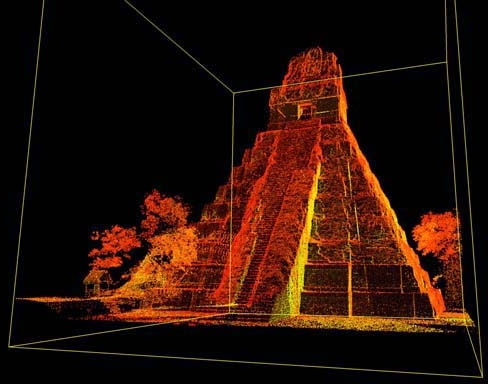
\includegraphics[width=0.5\textwidth]{localization_methods/lidar_scan}
	\caption{\gls{lidar} scan}
	\label{fig:localization-methods_lidar-scan}
\end{figure}

Given the high velocity in which light propagates, these methods allow the mapping of the environment with very low latency, which can be a critical requirement in robots that must react very fast to changes in their surroundings, such as autonomous cars [4].

\paragraph{Radio waves}

Similar to \gls{lidar}, radio waves can be used to calculate distances using the \gls{tof} technique. Systems like \gls{radar} provide an effective way to calculate the distance, altitude, direction and speed of objects that can be used as landmarks in navigation.

Like any electromagnetic wave localization method, it must take in consideration ambient interferences and even jamming, in order to validate the obtained measures. Moreover, some types of materials with a given geometric configuration might be invisible to RADAR, and as such, critical localization systems might have to employ some additional techniques to ensure the correct mapping of the robot surroundings.

Since RADAR has a less focused beam than \gls{lidar}, it can have considerable less accuracy, as can be seen in Figure 3. Nevertheless, it can be an effective method to avoid obstacles [5]

\paragraph{Sound waves}

Other localization approach that can be used to map under water environments relies in the acoustic analysis of the reflections of sounds in the surrounding objects.

Like the previous methods, \gls{sonar} can actively scan the environment to calculate the locations of the objects using a ToF technique (as can be seen in Figure 4). Although this method is usually applied to underwater mapping, it can also be used in other sound propagation environments, such as air [6].

\begin{figure}
	\centering
	\begin{minipage}[h]{.49\textwidth}
		\centering
		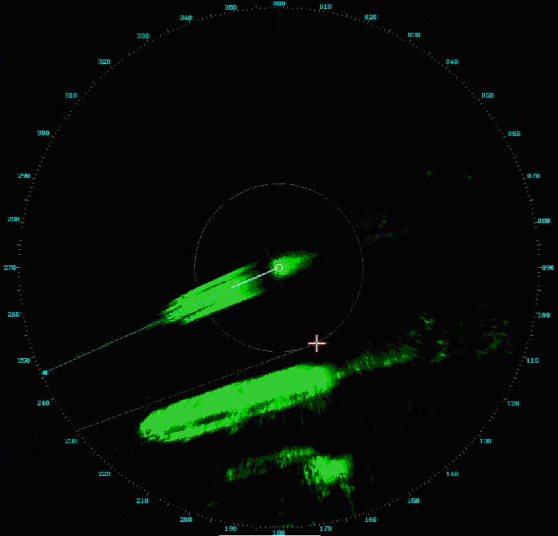
\includegraphics[width=\textwidth]{localization_methods/radar_scan}
		\caption{\gls{radar} scan of two ships}
		\label{fig:localization_methods_radar-scan}
	\end{minipage}\hfill
	\begin{minipage}[h]{.49\textwidth}
		\centering
		\includegraphics*[width=\textwidth]{localization_methods/sonar_scan}
		\caption{\gls{sonar} scan of two ships}
		\label{fig:localization_methods_sonar-scan}
	\end{minipage}
\end{figure}


\subsection{Trilateration methods}

Trilateration is a geometric technique that can be employed in the calculation of absolute or relative positions using distances from known points.

For 3D localization, it usually involves the intersection of 4 or more spheres, in which their radius is the distance to known positions.

\paragraph{ \gls{gnss}}

Global localization systems such as the \gls{gps} or \gls{glonass}, allow 3D localization in the planet Earth  using a trilateration method [7].

In these systems, a constellation of satellites broadcasts a radio signal with information about its position along with the time of the message dispatch. Using this data and knowing the speed of the radio waves, the distances to the satellites can be computed.

With at least 3 satellites distances, the 3D position can be calculated, since the Earth can be used as the 4${}^{th}$ sphere (Figure 5 shows a visual representation of the trilateration technique used in a global localization system).

Given that the correct measurement of the distances to the satellites relies in the accurate computation of the elapsed time between the message dispatch and its reception, it is critical that both the satellites and the receiver have synchronized clocks. This is achieved by using high precision atomic clocks in the satellites and a clock reset technique in the receiver. This reset technique relies on the fact that 3 satellite distances will only have a valid location if the clock of the receiver is synchronized. With this knowledge, the receiver can compute the necessary corrections to reset its internal clock to match the satellites time.

\begin{figure}[h]
	\centering
	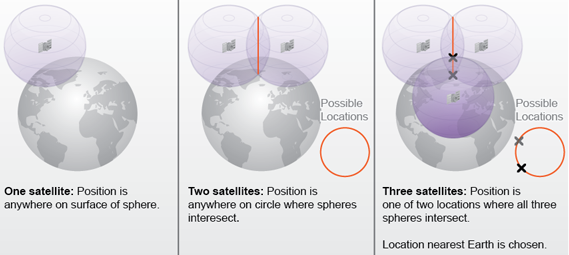
\includegraphics[width=\textwidth]{localization_methods/gnss}
	\caption{Trilateration technique in a global localization system}
	\label{fig:localization-methods_gnss}
\end{figure}

\paragraph{Differential Global Position System (DGPS)}

The accuracy of the GPS position can be increased with the help of local broadcast stations. These stations are fixed and provide information about the corrections that can be made to the satellite signals in order to improve the localization precision.

These corrections are useful to mitigate some of the ambient interference that the satellite signals face. These interferences can range from simple signal reflection in the environment landscape to the more complex interactions with the atmosphere, which can change the speed and path of the radio signals.

The computation of the corrections [8] is based on the fact that these stations are fixed, and as such, they can compare the location given by the satellite signals with their known location. With this position differential, the appropriate corrections can be calculated and broadcasted to the GPS receivers.

\paragraph{Assisted Global Positioning System (AGPS)}

AGPS systems are a common method used to speed up the Time To First Fix (TTFF) of a GPS receiver. They usually rely on the cellphone network to provide location estimation and signal corrections [9]. This information can greatly reduce the TTFF when there are few satellites visible or their signal is very weak and only temporary available.

\paragraph{Signal strength geolocation methods}

Signal strength geolocation [10], also known as fingerprinting localization [11], is an approximate method that can be used to calculate relative positions.

It relies on the analysis of the signal attenuation from a given access point (like a Wi-Fi router or cellphone tower), to estimate distances. With enough access points (usually 4), an approximate position can be computed.

This type of distance estimation can be useful for indoor navigation, but requires a propagation model of the signal and the environment. If these models aren't accurate, then the localization precision of these methods will be very low.

Although this method is less accurate than the more recent global localization systems (such as GPS), it can be used without human made infrastructures, and as such, is a viable solution in case of temporary disruption of the GPS signal.


\subsection{Celestial navigation}

Celestial navigation [12] relies on the observation of stars, planets or other reference objects, to calculate the latitude and longitude.

The calculation of the position on the surface of the Earth using celestial navigation is similar to trilateration, but in this case, angles are used instead of distances. These angles (delta), are measured between the Earth horizon and the center of the celestial object.

Having the delta, and knowing the relative position of the Earth to the reference object, along with the Greenwich hour time, it is possible to calculate a circle of position (as shown in Figure 6).

Having at least 3 circles of position, the latitude and longitude can be computed.

Although this method is less accurate than the more recent global localization systems (such as GPS), it can be used without human made infrastructures, and as such, is a viable solution in case of temporary disruption of the GPS signal.

\begin{figure}[h]
	\centering
	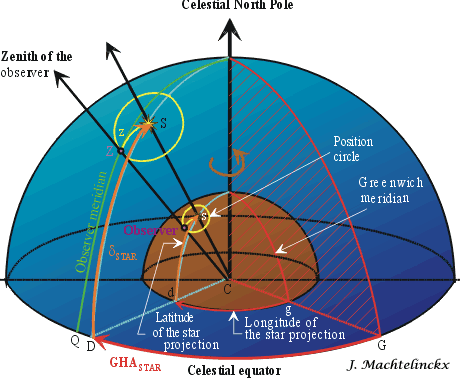
\includegraphics[width=\textwidth]{localization_methods/celestial_navigation}
	\caption{Circle of position in celestial navigation}
	\label{fig:localization-methods_celestial-navigation}
\end{figure}


\subsection{Landmark methods}

Landmark methods [13] can be used to perform relative localization, and are very useful to reduce the required information for navigation.

In these methods a database of markers / environment geometry is stored along with its location, and when the robot recognizes one of these markers, it corrects its proprioceptive methods measures.

It is a simplification of the method that will be presented in the next section, and it is useful for environments that have unique geometry in key positions of the navigation map.


\subsection{Point cloud methods}

Point cloud localization methods can be used to perform relative localization by finding the best point cloud match between the environment and the know map (Figure 7 shows its application to small objects). These methods require a 2D or 3D representation of the environment and tend to be used in conjunction with proprioceptive methods (to have an estimation of movement), and also with probabilistic methods (when the point cloud acquisition location is not known).

One of the most used algorithms for 3D point cloud matching is the Iterative Closest Point (ICP) [14]--[20]. It is an iterative algorithm that finds the translation and rotation transformations that minimizes the distances of the corresponding points on both clouds.

There are several variants that optimize different parts of the algorithm [21].

The main steps for each iteration of ICP algorithm are presented below.

\begin{enumerate}
\item  Selection of points in one or both point clouds (source and reference clouds)

\item  Matching / pairing source points to reference points

\item  Weighting the corresponding pairs

\item  Rejecting low quality matches (outliers)

\item  Assigning an error metric based on the point pairs

\begin{enumerate}
\item  Usually mean square error based on points distance
\end{enumerate}

\end{enumerate}


\begin{figure}[h]
	\centering
	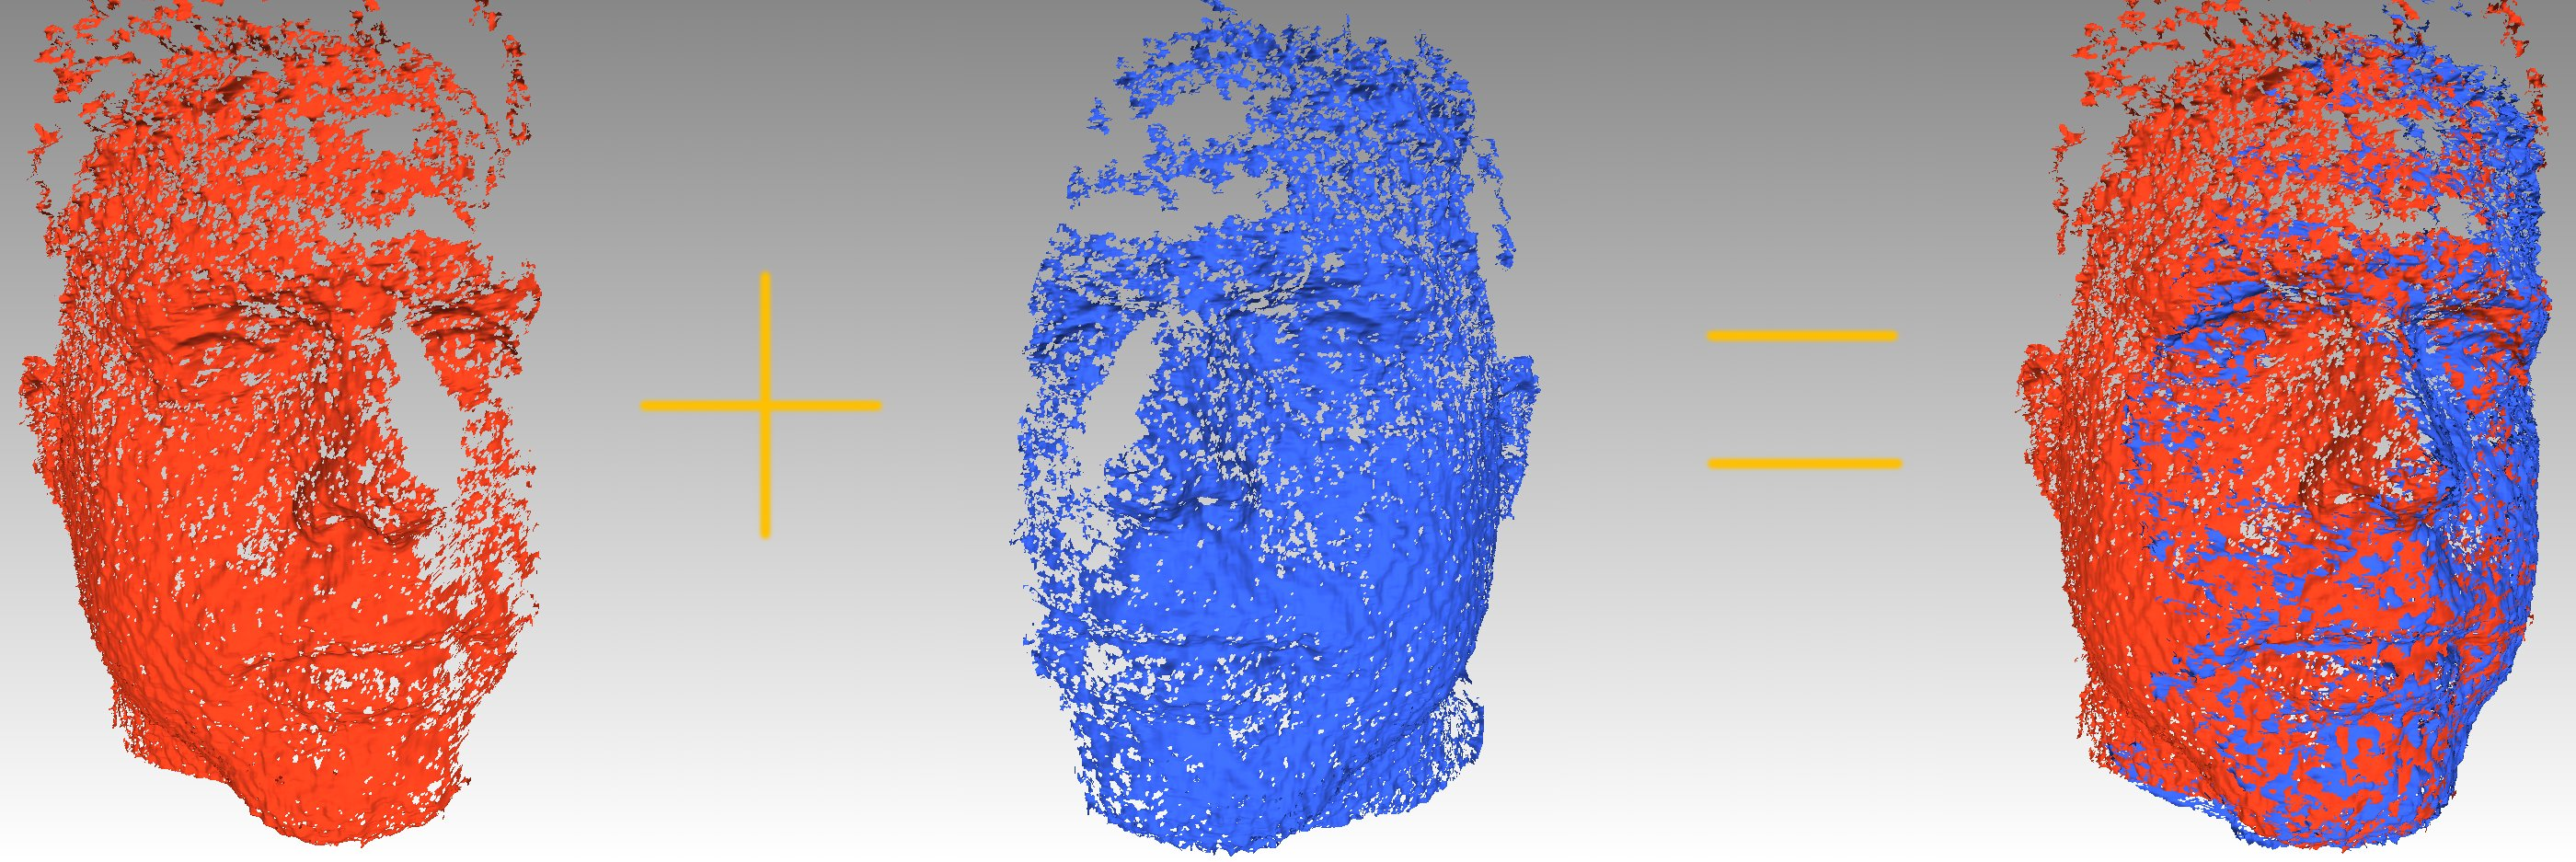
\includegraphics[width=\textwidth]{localization_methods/icp}
	\caption{ICP point cloud matching}
	\label{fig:localization-methods_icp}
\end{figure}


\subsection{Probabilistic methods}

Probabilistic methods aim to reduce the impact of sensor accumulated errors or even temporary malfunctions by using Bayesian estimations and Markov processes.

\paragraph{\gls{mcl}}

MCL (also known as particle filter), is a global localization algorithm that estimates the position and orientation of a robot by analyzing and adjusting the distribution and weights of state particles on a given environment [22]--[27].

It starts by randomly distributing the state particles on the map, and over time it changes their position and weight according to new sensor readings. The probable location of the robot will be in the area of the map that has the largest cluster of state particles.

The figures below shows the evolution of the state particles distribution during the robot movement in the environment, and illustrates how the new sensor readings changed the particles clusters [26].

\begin{figure}
	\centering
	\begin{minipage}[h]{.49\textwidth}
		\centering
		\animategraphics[width=\textwidth,loop,autoplay]{4}{localization_methods/mcl/frame-}{0}{39}
		\caption{\gls{mcl} particle distribution animation}
		\label{fig:localization-methods_mcl1}
	\end{minipage}\hfill
	\begin{minipage}[h]{.49\textwidth}
		\centering
		\includegraphics*[width=\textwidth]{localization_methods/mcl_2}
		\caption{\gls{mcl} redistribution of particles}
		\label{fig:localization-methods_mcl2}
	\end{minipage}
\end{figure}

\begin{figure}
	\centering
	\begin{minipage}[h]{.49\textwidth}
		\centering
		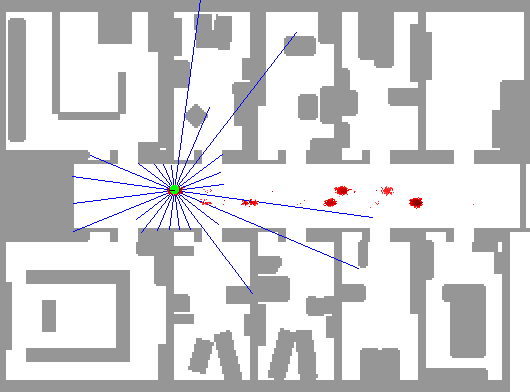
\includegraphics[width=\textwidth]{localization_methods/mcl_3}
		\caption{\gls{mcl} position refinement}
		\label{fig:localization-methods_mcl3}
	\end{minipage}\hfill
	\begin{minipage}[h]{.49\textwidth}
		\centering
		\includegraphics*[width=\textwidth]{localization_methods/mcl_4}
		\caption{\gls{mcl} position estimation}
		\label{fig:localization-methods_mcl4}
	\end{minipage}
\end{figure}


\paragraph{Kalman filters}

Kalman filters [28] are probabilistic algorithms that aim to estimate a given system state even when it is affected by noise or other errors. They perform linear quadratic estimations to achieve optimal results and can be efficiently implemented to be used in real time systems. They are recursive algorithms based on Marcov processes, and as a result, they only need to know the current system state in order to perform measurement corrections.

The Extended Kalman Filter (EKF) [29]--[32] is a variant of the Kalman filter, designed to handle non-linear systems by performing linear approximations to the state variables. These approximations may lead to divergence in the estimations, and as such, the EKF can't guarantee optimal results.

The Unscented Kalman Filter (UKF) [33], [34] is another variant of the Kalman filter that was designed for highly non-linear systems. It usually achieves better results than EKF due to its unscented transform.

For the particular case of localization, these algorithms start with an initial estimation of the system state, and for each new position (computed from the sensors data), they predict the estimated robot location (according to the Bayes estimation model and the Gaussian distribution of errors), and then update their internal model of the system (mean and covariance) to incorporate the system evolution.

In \cref{fig:localization-methods_ukf} can be seen that the UKF estimated position (red) is closer to the real position (blue) than the raw sensor measurements (green).

\begin{figure}[h]
	\centering
	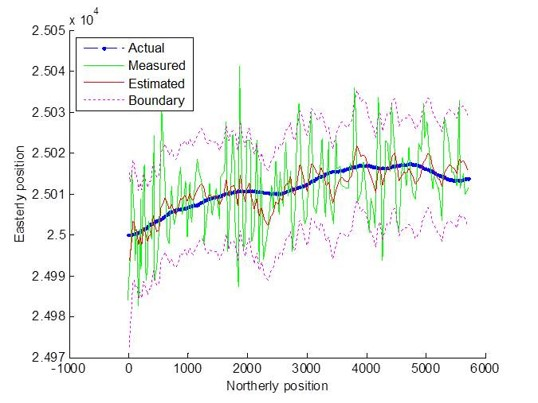
\includegraphics[width=\textwidth]{localization_methods/ukf}
	\caption{Unscented Kalman Filter}
	\label{fig:localization-methods_ukf}
\end{figure}

\paragraph{Perfect Match}

The Perfect Match [35], [36] is an efficient self-localization algorithm that is largely used in the Robocup Robotic Soccer Midsize League. Its main goal is to minimize the localization error by carefully analyzing the know map, and selecting the most probable current position using a gradient descent approach. To improve tracking accuracy, the algorithm also uses a stochastic weighted approach.

With the proper configuration, it can achieve a localization accuracy similar to the particle filter, while using about ten times less computations.

An example of the position estimation can be seen in the figures below. Figure 13 shows the probable locations when the robot detects a line on the floor, and Figure 14 illustrates their associated errors (brighter areas indicate smaller error). By using a gradient descent, the most probable location was selected (black circle).

\begin{figure}
	\centering
	\begin{minipage}[h]{.49\textwidth}
		\centering
		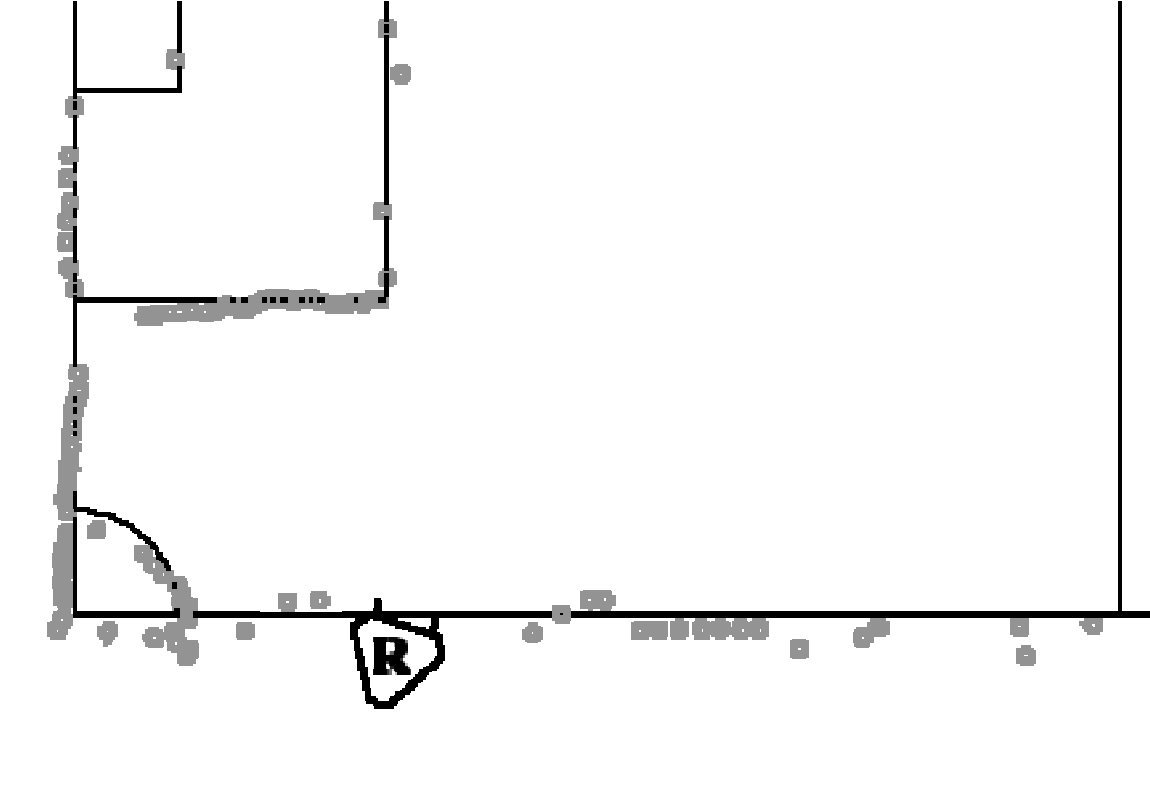
\includegraphics[width=\textwidth]{localization_methods/pm_1}
		\caption{Position estimates}
		\label{fig:localization-methods_pm-1}
	\end{minipage}\hfill
	\begin{minipage}[h]{.49\textwidth}
		\centering
		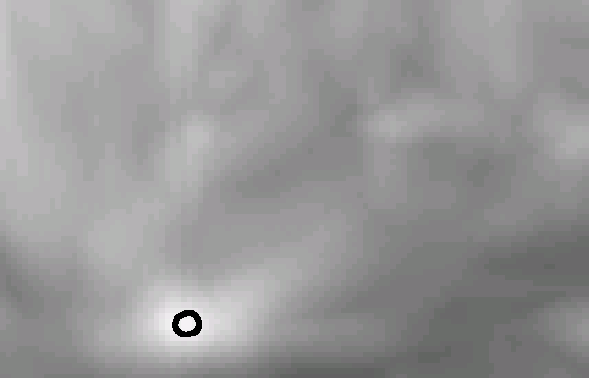
\includegraphics[width=\textwidth]{localization_methods/pm_2}
		\caption{Positions associated error}
		\label{fig:localization-methods_pm-2}
	\end{minipage}
\end{figure}


\subsection{\gls{slam}}

SLAM [37] is a very effective approach to either explore unknown environments or update a known map. It relies on both proprioceptive and exteroceptive methods to perform localization and mapping.

It is also very useful to make the robot navigation more robust in dynamic environments, in which the topology of the world may change considerably over time.

There are numerous approaches to perform  SLAM [38]. Some optimized for exploration and others for map improvement.

For the exploration tasks, proprioceptive methods play a critical role, and are usually paired with probabilistic methods, such as Kalman filters, in order to reliably map the environment.

For map correction and improvement, several probabilistic methods can be employed according to the precision required. For high accuracy 3D mapping, the ICP algorithm can be used to build accurate point clouds of the environment.



\section{Summary}

This chapter introduced several localization systems that can be used in different types of environments and with different degrees of accuracy. It started with the simple proprioceptive methods and then moved on to the more robust exteroceptive approaches.

Some techniques can be combined to improve the pose estimate or to make the localization more efficient to a particular type of environment.

For outside tasks, a GNSS approach can give accurate localization estimations with very little computation cost. On the other hand, indoor localization requires more advanced techniques in order to infer the current position based on the analysis of the robot surroundings. These techniques usually start with an estimation of the robot movement and then refine it with probabilistic or geometric methods.

Table 1 presents an overview of the mentioned localization techniques.

